\documentclass[11pt,a4paper,titlepage]{article}
\usepackage{graphicx}
\DeclareGraphicsExtensions{.png}
\DeclareGraphicsExtensions{.jpg}

\begin{document}
\begin{titlepage}
	\begin{center}
		
		\begin{figure}[t]
			\centering
			
\includegraphics[width=350px, height=7cm]{images/thinkTechLogo.jpg}
		\end{figure}	
	
	\begin{flushright} 
		
		\textbf{\LARGE COS301 Main Project}
		\newline \newline \newline
		\textbf{\LARGE Flowchart Simulation Tool User Manual}
		\newline \newline \newline
 		\textbf{\LARGE ThinkTech}
		\newline \newline
	\end{flushright}
	
	\begin{flushright} \large
			
			\textbf{\LARGE Stakeholders}\newline 
			Lelethu Zazaza 13028023\newline
			Goodness Adegbenro 13046412\newline
			Hlavutelo Maluleke 12318109\newline
			Tshepiso Magagula 12274195\newline
			Xoliswa Ntshingila 13410378\newline
			
			
	\end{flushright}
	
	\begin{flushright} \large
	
			\textbf{\LARGE Client}\newline 
			Mr Willem S. van Heerden \newline
			University of Pretoria (Junior Lecturer)\newline
			
	\end{flushright}
		
		\vspace{1 cm}
		

		
		\vfill
		
		{\LARGE Version 0.2}
		\\
		{\large \today}		
		
		
	\end{center}
\end{titlepage}


\newpage
\tableofcontents
\pagenumbering{roman}
\newpage
\pagenumbering{arabic}
\section{General Information}
	\subsection{System Overview}
	
		Flowchart Simulation Tool is an application which allows for designing and executing flowchart diagrams. This application is intended for academic purposes for students with basic knowledge of programming design and implementation. This is a platform where the students can construct their own flowcharts, test and use them as they would like. \newline
		
		Furthermore, the system can be used in the commercial industry for various purposes.
		
\section{System Summary}
	\subsection{System Configuration}
		
		The flowchart tool is intended to operate on any Linux distribution. However, it can also be used on Windows and Mac OS. It is not a very sophisticated software, not so many configurations required.
		
		Any version of Java should be installed to allow for successful execution of the program. 
		
		\subsection{System Installation}
		
		This system is a "plug-and-play" type of application, for which the executable file can be found from the University of Pretoria (Computer Science) website.
		

\section{Getting Started}
	
	For one to get to use the system, that particular user must be registered at the University of Pretoria, and have access to the Linux platform which is granted by the Department of Computer Science. From Linux, the user must be able to access the application, without any further installation or signing-up required.







% This section forms the bulk of the user manual.








	
	\subsection{Running Software}
		The application will not require any installation. To run the application the user will only require the executable file which will be provided via the on-line University of Pretoria (Computer Science) website. With the executable file the user will only need to double click on the file, then the system will star-up.
		
		\subsection{Software Layout}
		The layout is composed of the canvas, flowchart tools and menu options. \newline 
		The figure below depicts the general layout of the entire system. \newline \newline
		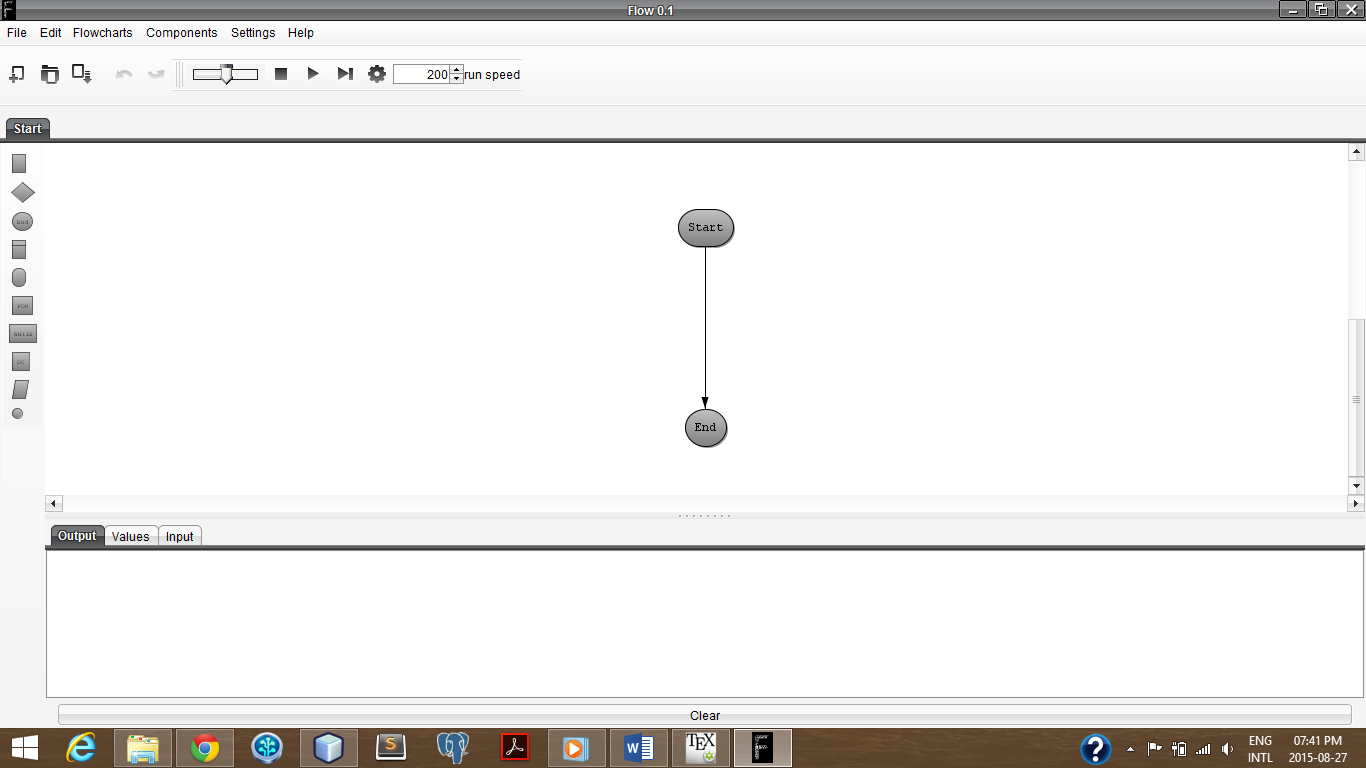
\includegraphics[width=\textwidth]{SystemLayout.jpg}
		\begin{center}
		Figure: The General System Layout.\newline
		\end{center}
		
		
		\begin{itemize}
			\item \textbf{Canvas:} This space is provided to design a 			well-formed flowchart. Components will be dragged from the flowchart 				tools menu consisting of available components and dropped onto the 				canvas. See figure below.\newline
			There are components which are already implemented at start of the system, the 'start' and 'end' blocks are initialised by default on the canvas.\newline \newline
			
\includegraphics[width=11.5cm]{Canvas.jpg}
			\begin{center}
		Figure: The Canvas.\newline
		\end{center}
			
			\item \textbf{Flowchart Tools:} This contains all the tools required to construct the flowchart. All the components will be dragged and dropped onto the canvas (as illustrated by the the figure below), with the tools on the left and the canvas on the right. All the necessary components to build a flowchart are listed on the left toolbar.\newline \newline
			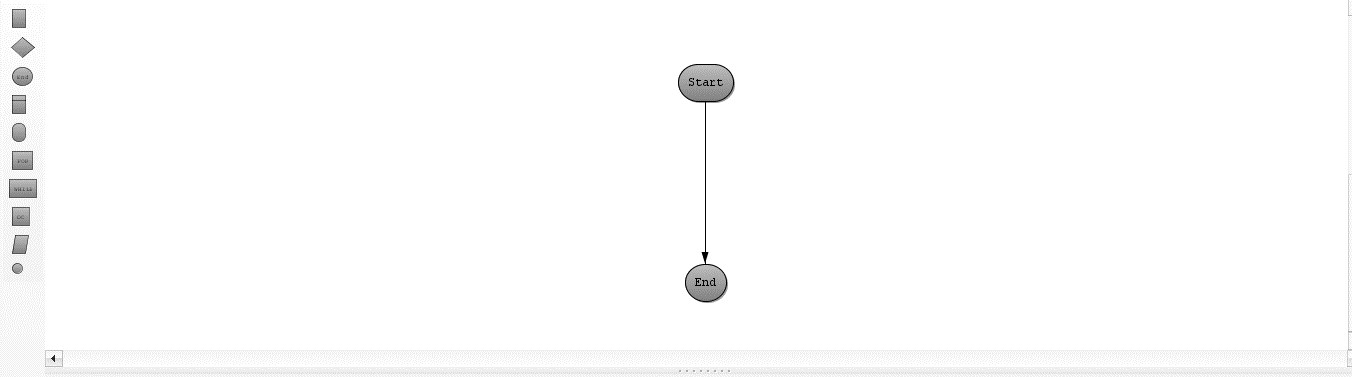
\includegraphics[width=11.5cm]{Tools.jpg}
			\begin{center}
		Figure: Flowchart Tool Components.\newline
		\end{center} 
			
						
			\item \textbf{Menu Options -} The menu option provides options of creating, saving, deleting and loading projects onto the canvas. Also, this provides the user with many more options which are accessible by hovering over the name of the option. The figure below shows the functionality of all this.\newline \newline
			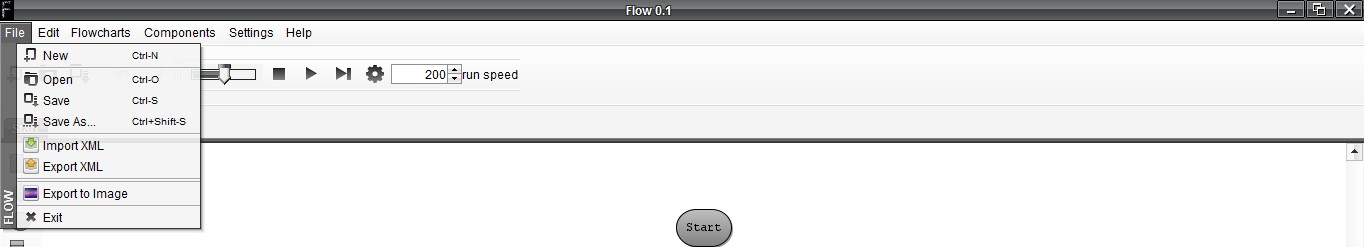
\includegraphics[width=11.5cm]{Menu.jpg}
			\begin{center}
		Figure: Menu Bar.
		\end{center}
			
			
		\end{itemize}

	\newpage
	
	
	
%%%%%%%%%%%%%%%%%% Very important %%%%%%%%%%%%%%%%%%%%%%%%%%%%%%%%%%%%%%
	
	
	
\section{Using the System}
	\subsection{Creating New Project}
	
	When the application is opened for the first time, a default project is created with a default flowchart, which compiles and execute without any output generated. The user then will start his/her own building of the flowchart from already generated default flowchart. This is also demonstrated by the figure on general flowchart layout. \newline\newline
However, the user can create new project from the menu bar. To create a new project select "File" in the menu bar and a drop down menu will appear. Select the "New" option, a pop-up window will appear requesting the desired file name for the project. Enter the file name and press the enter key on the keyboard, then the new project with the default flowchart will be created. \newline
		
		
	\subsection{Adding Components to Canvas}
	
	From the created project, construction starts with dragging the components from the tool bar to the canvas. Adding components to the canvas is quite simple, drag the desired component from the tool bar and drop it onto the canvas. The component will be locally saved on the canvas, continue doing so until the building is complete.
	
	\subsection{Editing Component}
	
	Editing the component entails manipulation of the features and adding code inside the component. To edit the component click on the component that you want to edit and the a pop-up window will appear on the far left side of the application with the options of changing features or adding code.
		
	\subsection{Removing Components from Canvas}
	
	To remove any component from the canvas right-click on the component and select delete component. To remove multiple components hold the "SHIFT" key and select the components and then right-click and select delete component.
		
	\subsection{Saving Project}
	
	To save your current progress go to "File" in the menu bar, in the drop down menu select "Save". Enter the name of the file and then the project will be saved in a directory for flowchart projects.
	
	\subsection{Run Simulation}
	To run the flowchart select the "Run" icon on the flowchart tools window and the the whole flowchart will execute. To run the flowchart step-by-step select the "Step" icon.
	
		
	\subsection{Opening Existing Project}
	
	To open an existing project go to the menu bar and select the "File" option and then select the "Open" menu item. Search for an existing flowchart project with the valid extention. The flowchart project will now be loaded onto the canvas and should be able to be updated.
	
\section{Troubleshooting}

This system is not connected to any other external systems, this reduces the amount of errors that might usually breakdown the system.

\end{document}